\subsection{On-set and Dailies -- Apple iPad Review} \label{subsec:ff-onset-dailies-ipad}

	\subsubsection{Summary}
	
	Dailies generation and review is a critical step in the motion picture production process.  Reviewing takes, making edit decisions, and sharing that information with editorial and post-production is often a task completed with Apple iPads.  Ensuring accurate color reproduction of dailies can aid in the decision making process. The following is a recommendation for the usage of output device transforms for dailies review using Apple iPads.
	
	\subsubsection{Workflow}
	
	The complete workflow from camera to dailies is beyond the scope of this document, but Figure \ref{fig:workflow3} shows a typical workflow for the creation and review of dailies on an Apple iPad during feature film production.
	
	\begin{figure*}[ht!]
	\centering
	    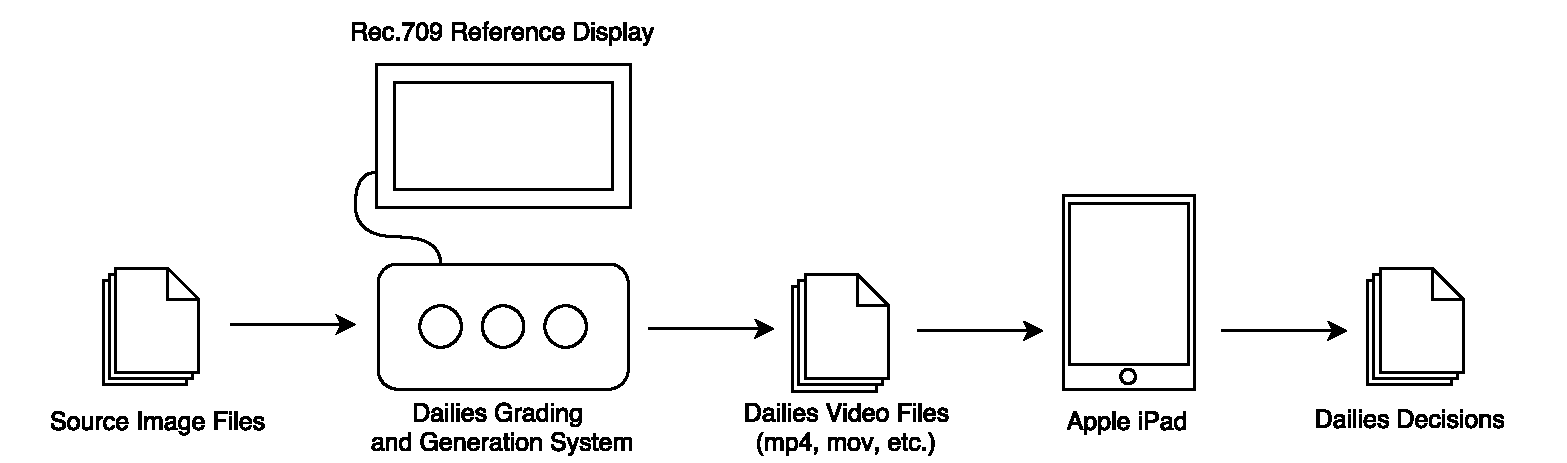
\includegraphics[width=4in]{images/workflows/workflow_ff-onset-dailies-ipad.pdf}
	    \caption{\small Feature Film On-set and Dailies -- iPad Review}
	    \label{fig:workflow3}
	\end{figure*}
	
	In this dailies review workflow images captured on-set are passed to a dailies generation system.  The dailies generation system is used to organize the captured image data based on scenes, takes, etc. and optionally basic grades may be applied based on the directors instructions or look data captured from an on-set look generation system. These basic grades are typically viewed on a Rec.709 reference display attached to the dailies grading and generation system.  After the images have been appropriately cataloged and the basic grades have been applied they are exported as Rec.709 encoded video files (mp4, mov, etc.) for the director's review.  These video files often are viewed on an Apple iPad using specialized software that aids in the capture of dailies review decisions.
	
	\begin{table}[ht!]
	\centering
	\begin{tabular}{|p{0.5in}|p{1.2in}|p{3.75in}|}
	\hline
	\textbf{System}   & \textbf{Display}            & \textbf{Suggested ODT}                                                  \\ \hline
	Dailies System Display & Rec.709 Reference Monitor   & \texttt{\seqsplit{ODT.Academy.Rec709\_D60sim\_100nits\_dim.a1.0.3}} \\ \hline
	Dailies Review Device & Apple iPad & \texttt{\seqsplit{ODT.Academy.Rec709\_D60sim\_100nits\_dim.a1.0.3}}           \\ \hline
	\end{tabular}
	\caption[Workflows - Feature Film (On-set and Dailies) - Suggested ODTs]{Summary of suggested ODTs}
	\label{tab:sum-ff-onset-dailies-ipad}
	\end{table}
	
	\subsubsection{Discussion}
	
	The dailies generation systems should have the ability to apply ACES color management, including an ODT to the source images files.  For review on the device the \texttt{\seqsplit{ODT.Academy.Rec709\_D60sim\_100nits\_dim.a1.0.3}} ODT should be used assuming the device includes a Rec.709 Reference Display.  Care should be taken to insure that the dailies generation system and attached Rec.709 Reference Display are properly calibrated and in a dim surround viewing environment.  
	
	Video files intended for review on an Apple iPad should be exported from the dailies system using the \texttt{\seqsplit{ODT.Academy.Rec709\_D60sim\_100nits\_dim.a1.0.3}} ODT.  The Apple iPad includes its own ACES-independent color management system.  As such, care should be taken to generate Rec.709 encoded video files (mp4, mov, etc.) from the dailies system.  Key to proper display of the video files is proper metadata tagging.  In particular, Apple's video color management system requires the \texttt{nclc} tag be present and correctly set.  The \texttt{nclc} should be set to \texttt{1-1-1} to inform Apple's video color management that the video files are encoded according to Rec.709 so that the proper color matrix, YCbCr to RGB conversion, and transfer function are applied.  It's critical to note that \texttt{1-1-1} is not the assumed value for the \texttt{nclc} tag if it is not present.  If the \texttt{nclc} tag is omitted or set to a value other than \texttt{1-1-1} by the dailies generation system, the video files will be displayed incorrectly on the Apple iPad.